\chapter{Specimen Collection}

The \entitytarget{Participant} aggregate is used to record specimens collected
from study participants. Before specimen collection can be recorded, the
participant must be created. Participants cannot be added to a
\entitylink{Study} that is not enabled.

A participant has a unique identifier that is used to identify the participant
in the system. This identifier is not the same as the
\valobjlink{ParticipantId} value object used by the domain model.

Figure \ref{fig:participant-aggregate} shows the composition of this aggregate.

\begin{figure}[H]
  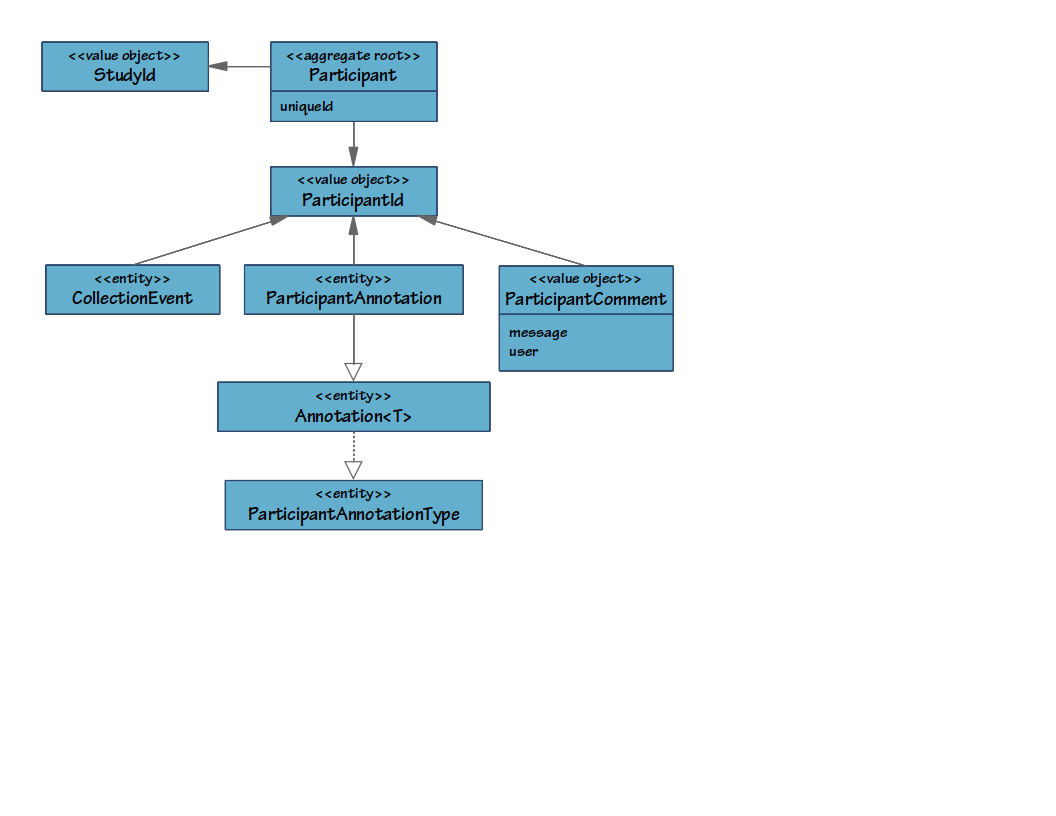
\includegraphics[trim={10mm 75mm 102mm 10mm}, clip,
    width=0.75\textwidth]{images/participant-aggregate}
  \caption{Participant aggregate}
  \label{fig:participant-aggregate}
\end{figure}

\subsection*{CollectionEvent}
Represents a visit made by a \entitylink{Patient} during which
\entitylink{Specimen}s may have been collected and other information may have
been recorded.

\subsection*{ParticipantAnnotation}
This entity holds the annotation value for the annotation type defined in the
study. For a single annotation, the value is the field listed below depending
on the annotation type's \texttt{valueType} (see Section
\ref{sec:participant-annotations}). The unused fields are assigned the
\texttt{null} value.

\begin{table}[!htbp]
\renewcommand{\arraystretch}{1.1}
\begin{tabularx}{\textwidth}{l l}
  \sffamily{\textbf{ValueType}} & \sffamily{\textbf{Value field}}\\
  \hline
  String & \texttt{stringValue}\\
  Number & \texttt{numberValue}\\
  Date & \texttt{numberValue} and stored as number of seconds\\
  Select & \texttt{selectedValue}\\

\end{tabularx}
\end{table}

\subsection*{ParticipantComment}
A \entitytarget{ParticipantComment} contains a textual message and the user
that added the comment. The date and time the comment was made is recorded as
meta data. A participant can have one or more comments.

\section{CollectionEvent Details}

\begin{figure}[H]
  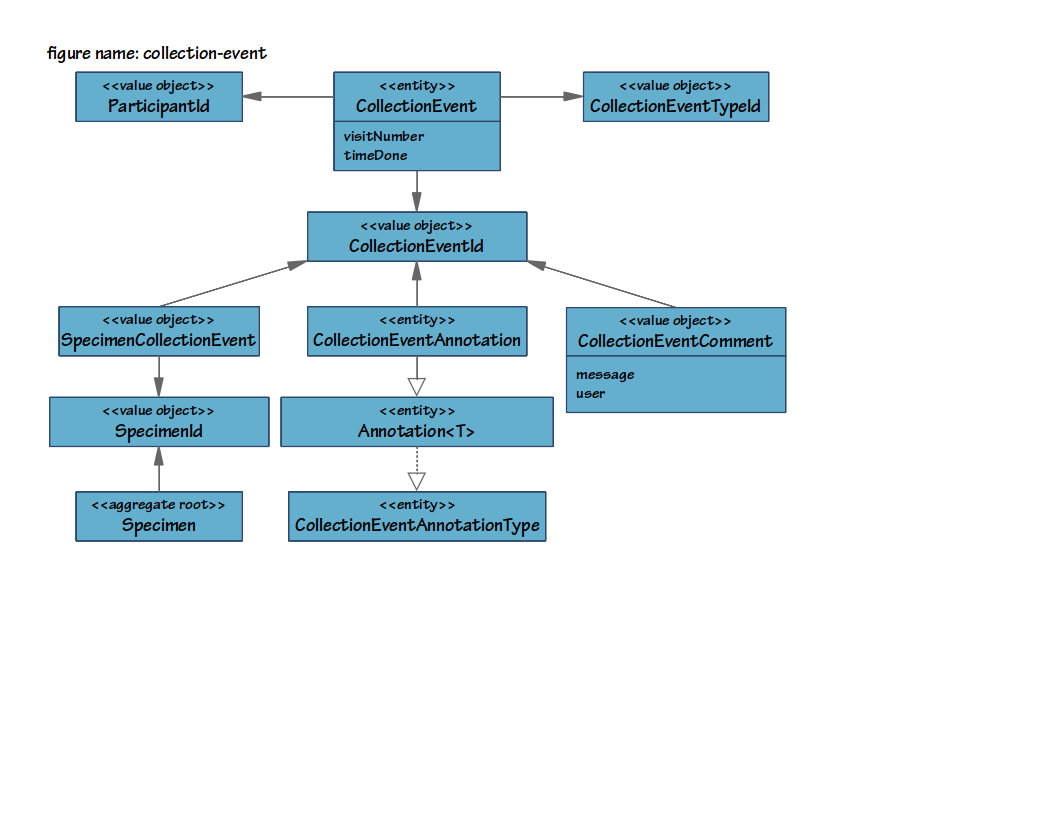
\includegraphics[trim={10mm 66mm 75mm 10mm}, clip,
    width=0.85\textwidth]{images/collection-event}
  \caption{CollectionEvent entity}
  \label{fig:collection-event}
\end{figure}
